\section{Anhang}\label{anh}

\begin{figure}[!h]
\centering
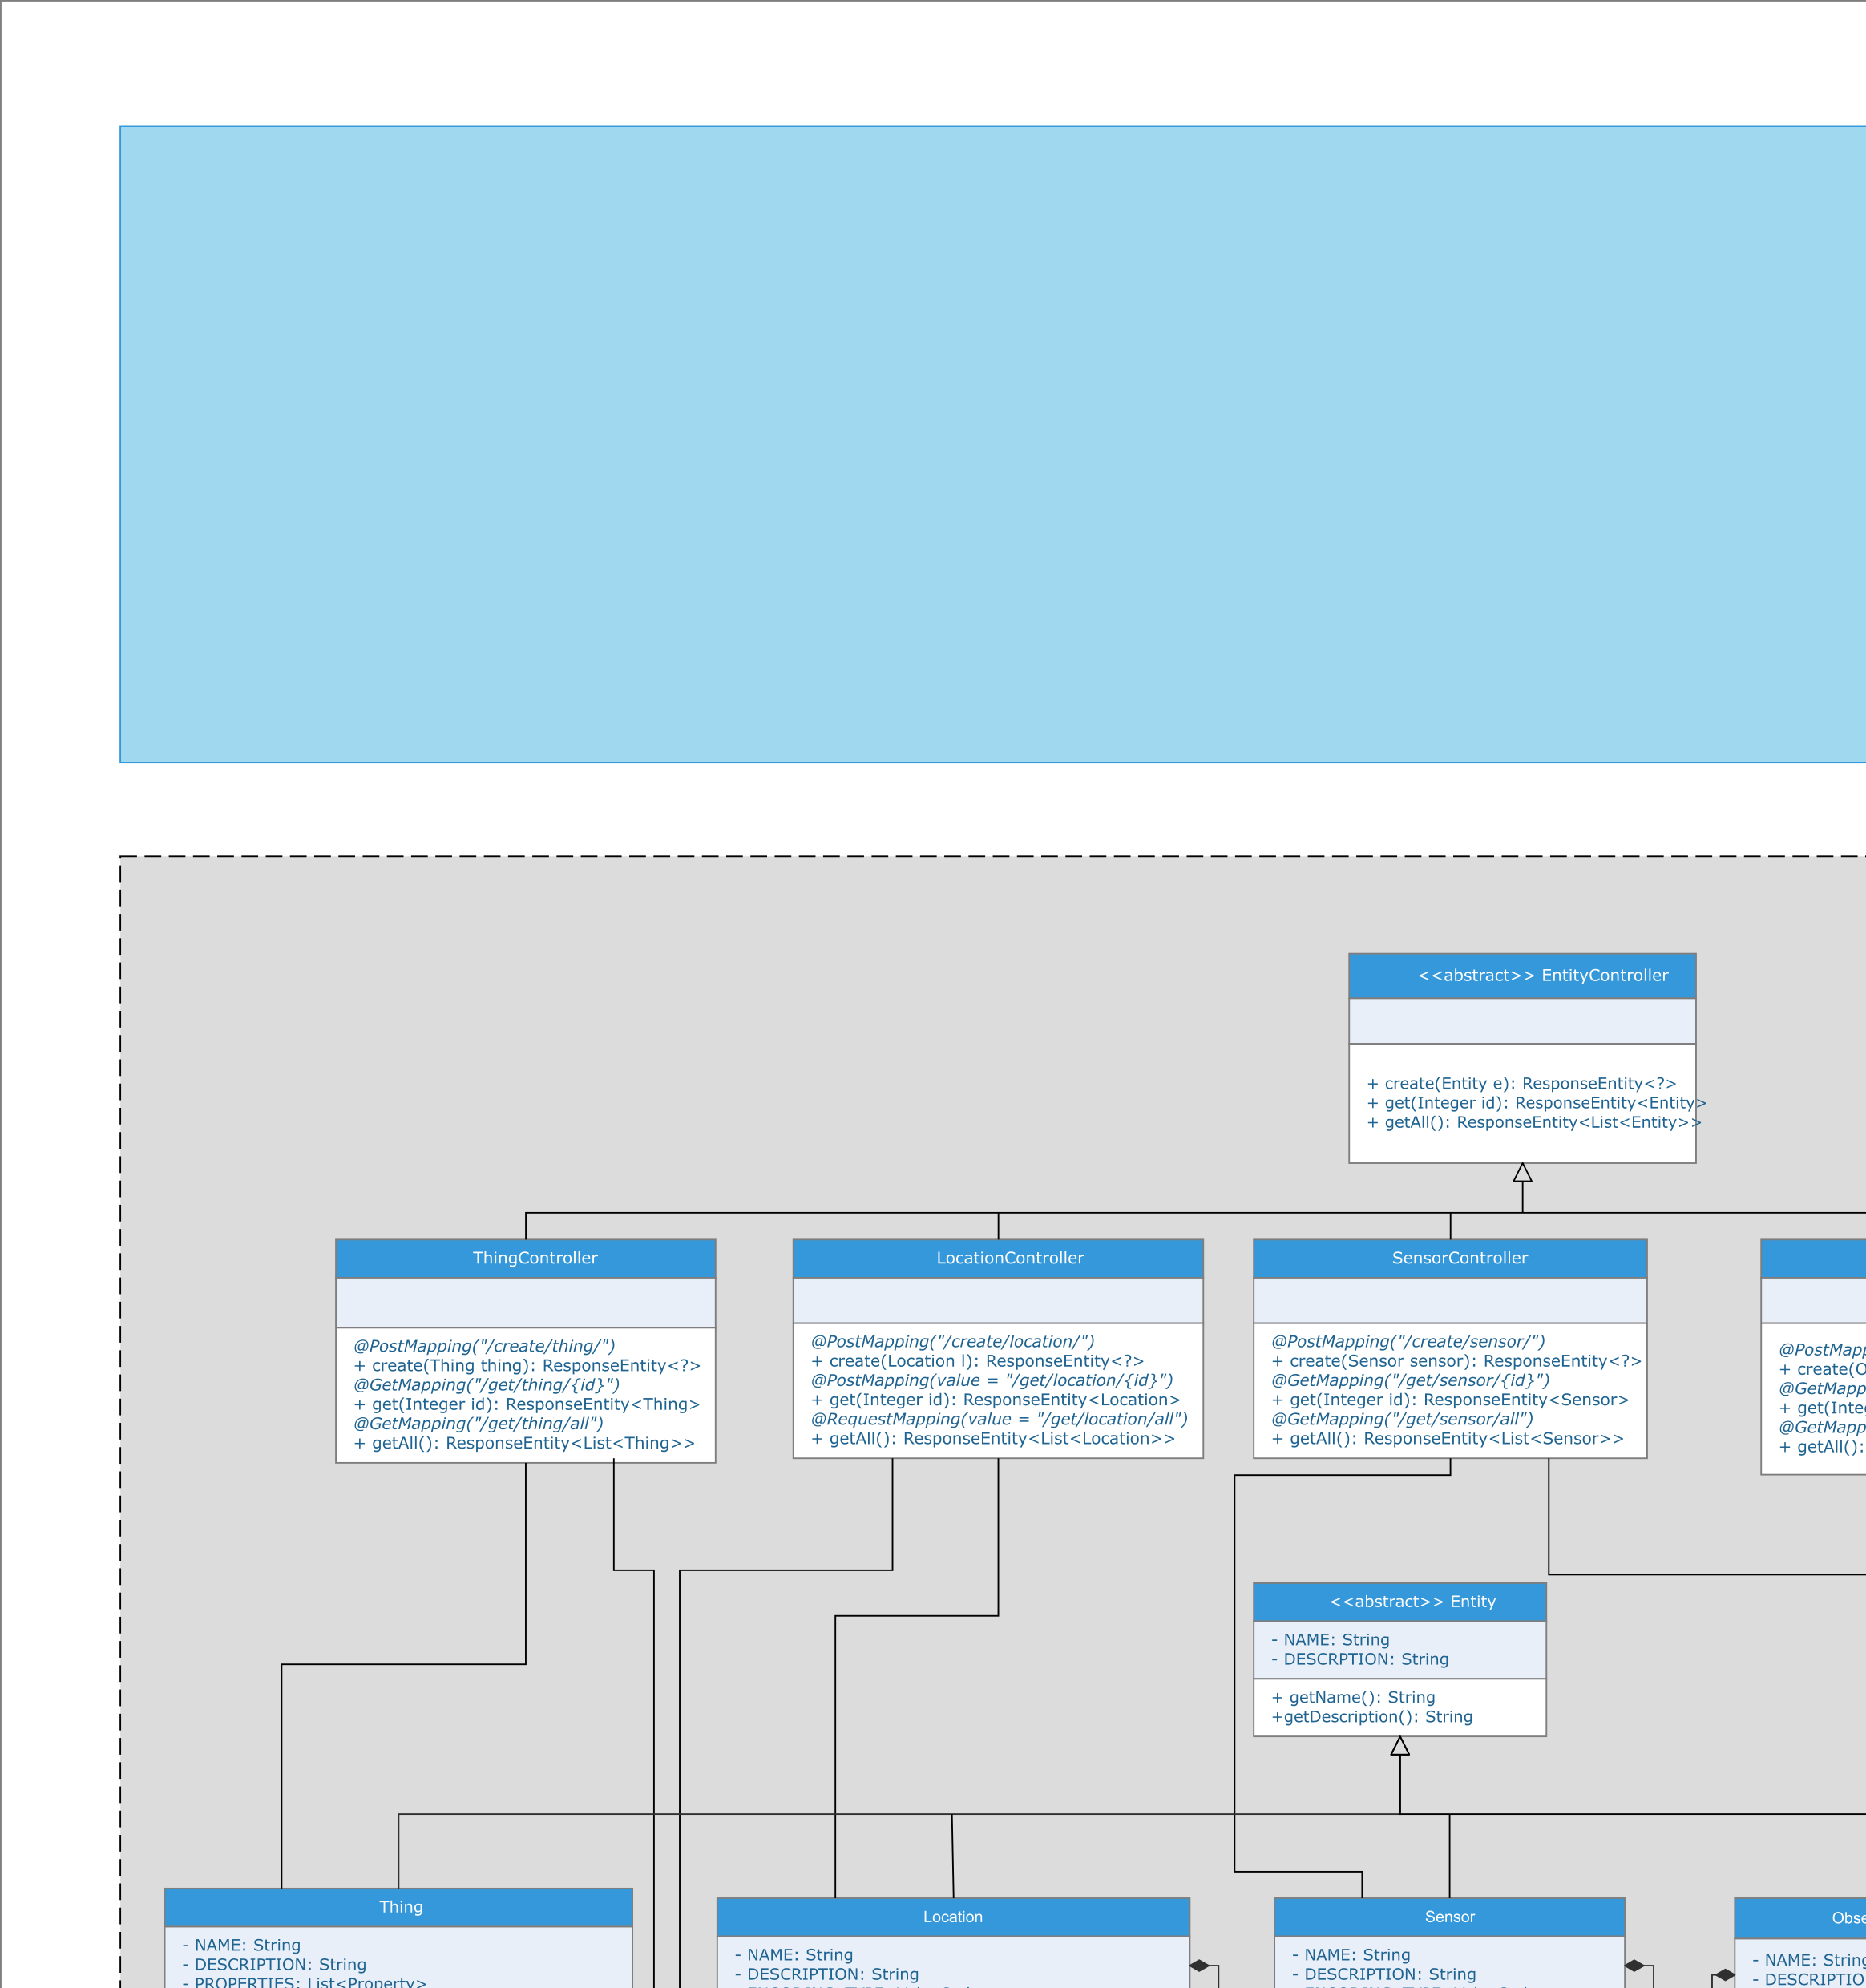
\includegraphics[scale=0.4]{uml/screenshots/frithjof/slice_0_0}
\caption{Ausschnitt 1 des Klassendiagramms}
\end{figure}
\clearpage

\begin{figure}[!h]
\centering
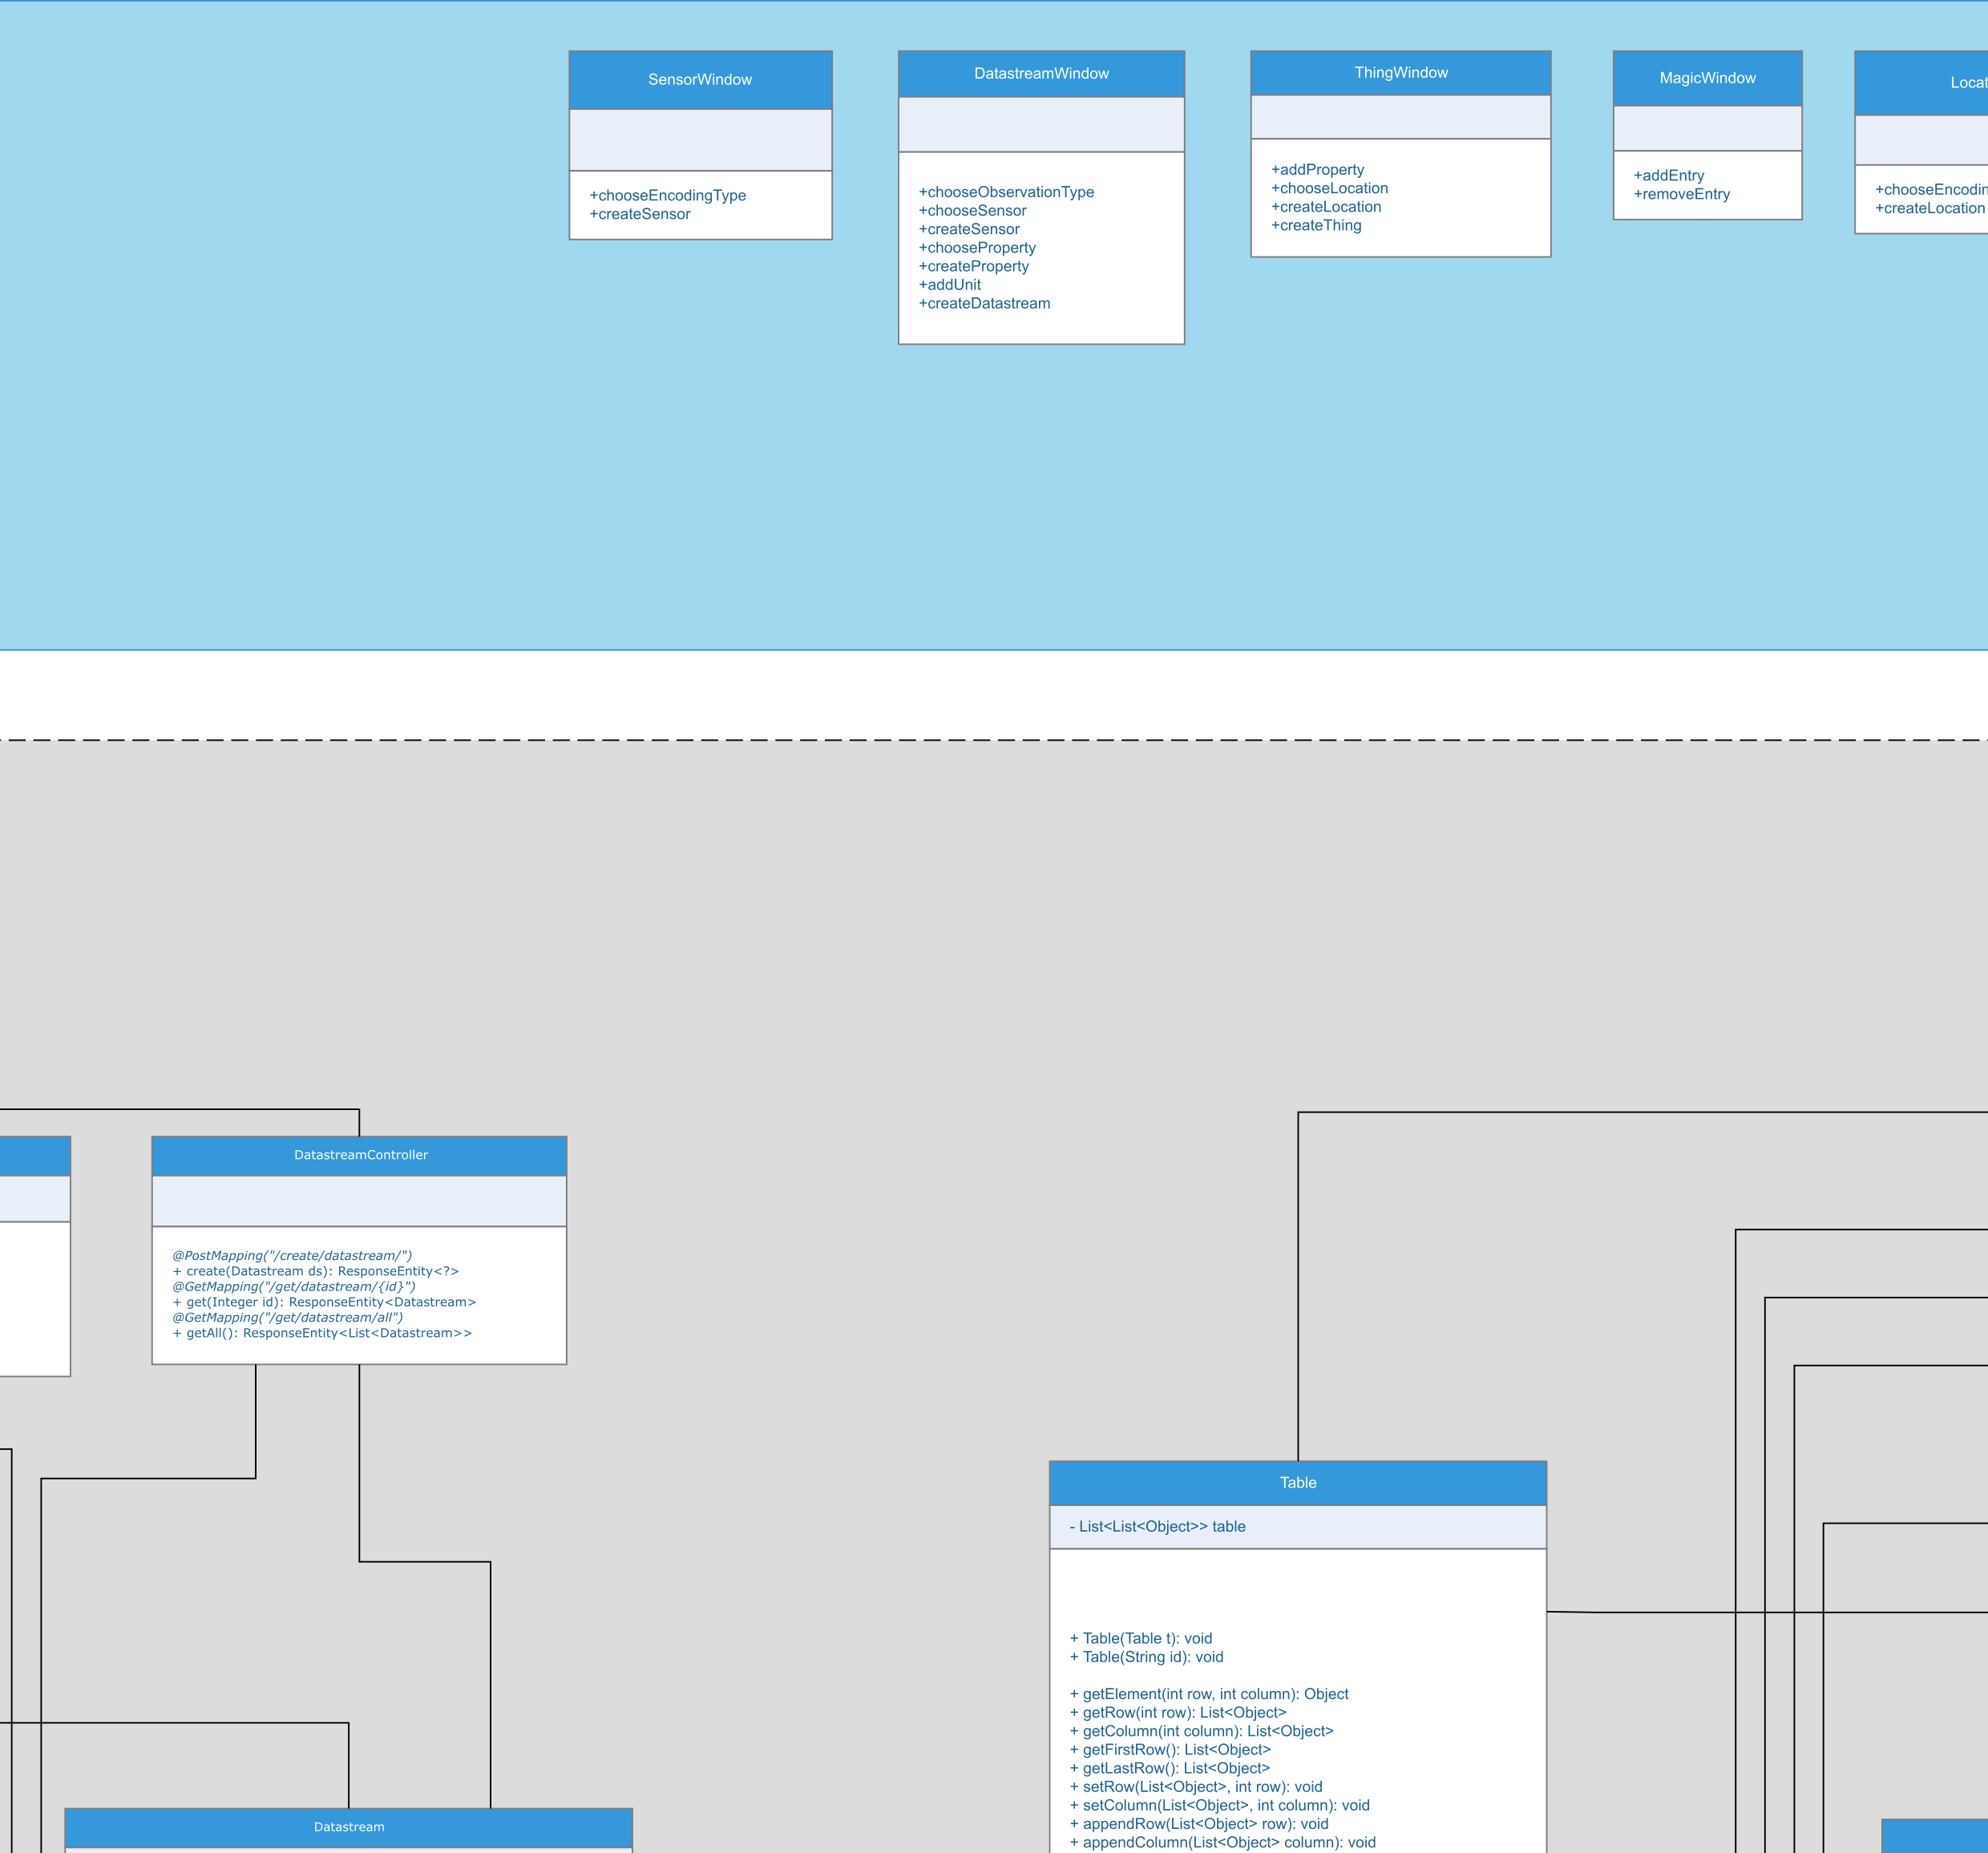
\includegraphics[scale=0.4]{uml/screenshots/frithjof/slice_0_1}
\caption{Ausschnitt 2 des Klassendiagramms}
\end{figure}
\clearpage

\begin{figure}[!h]
\centering
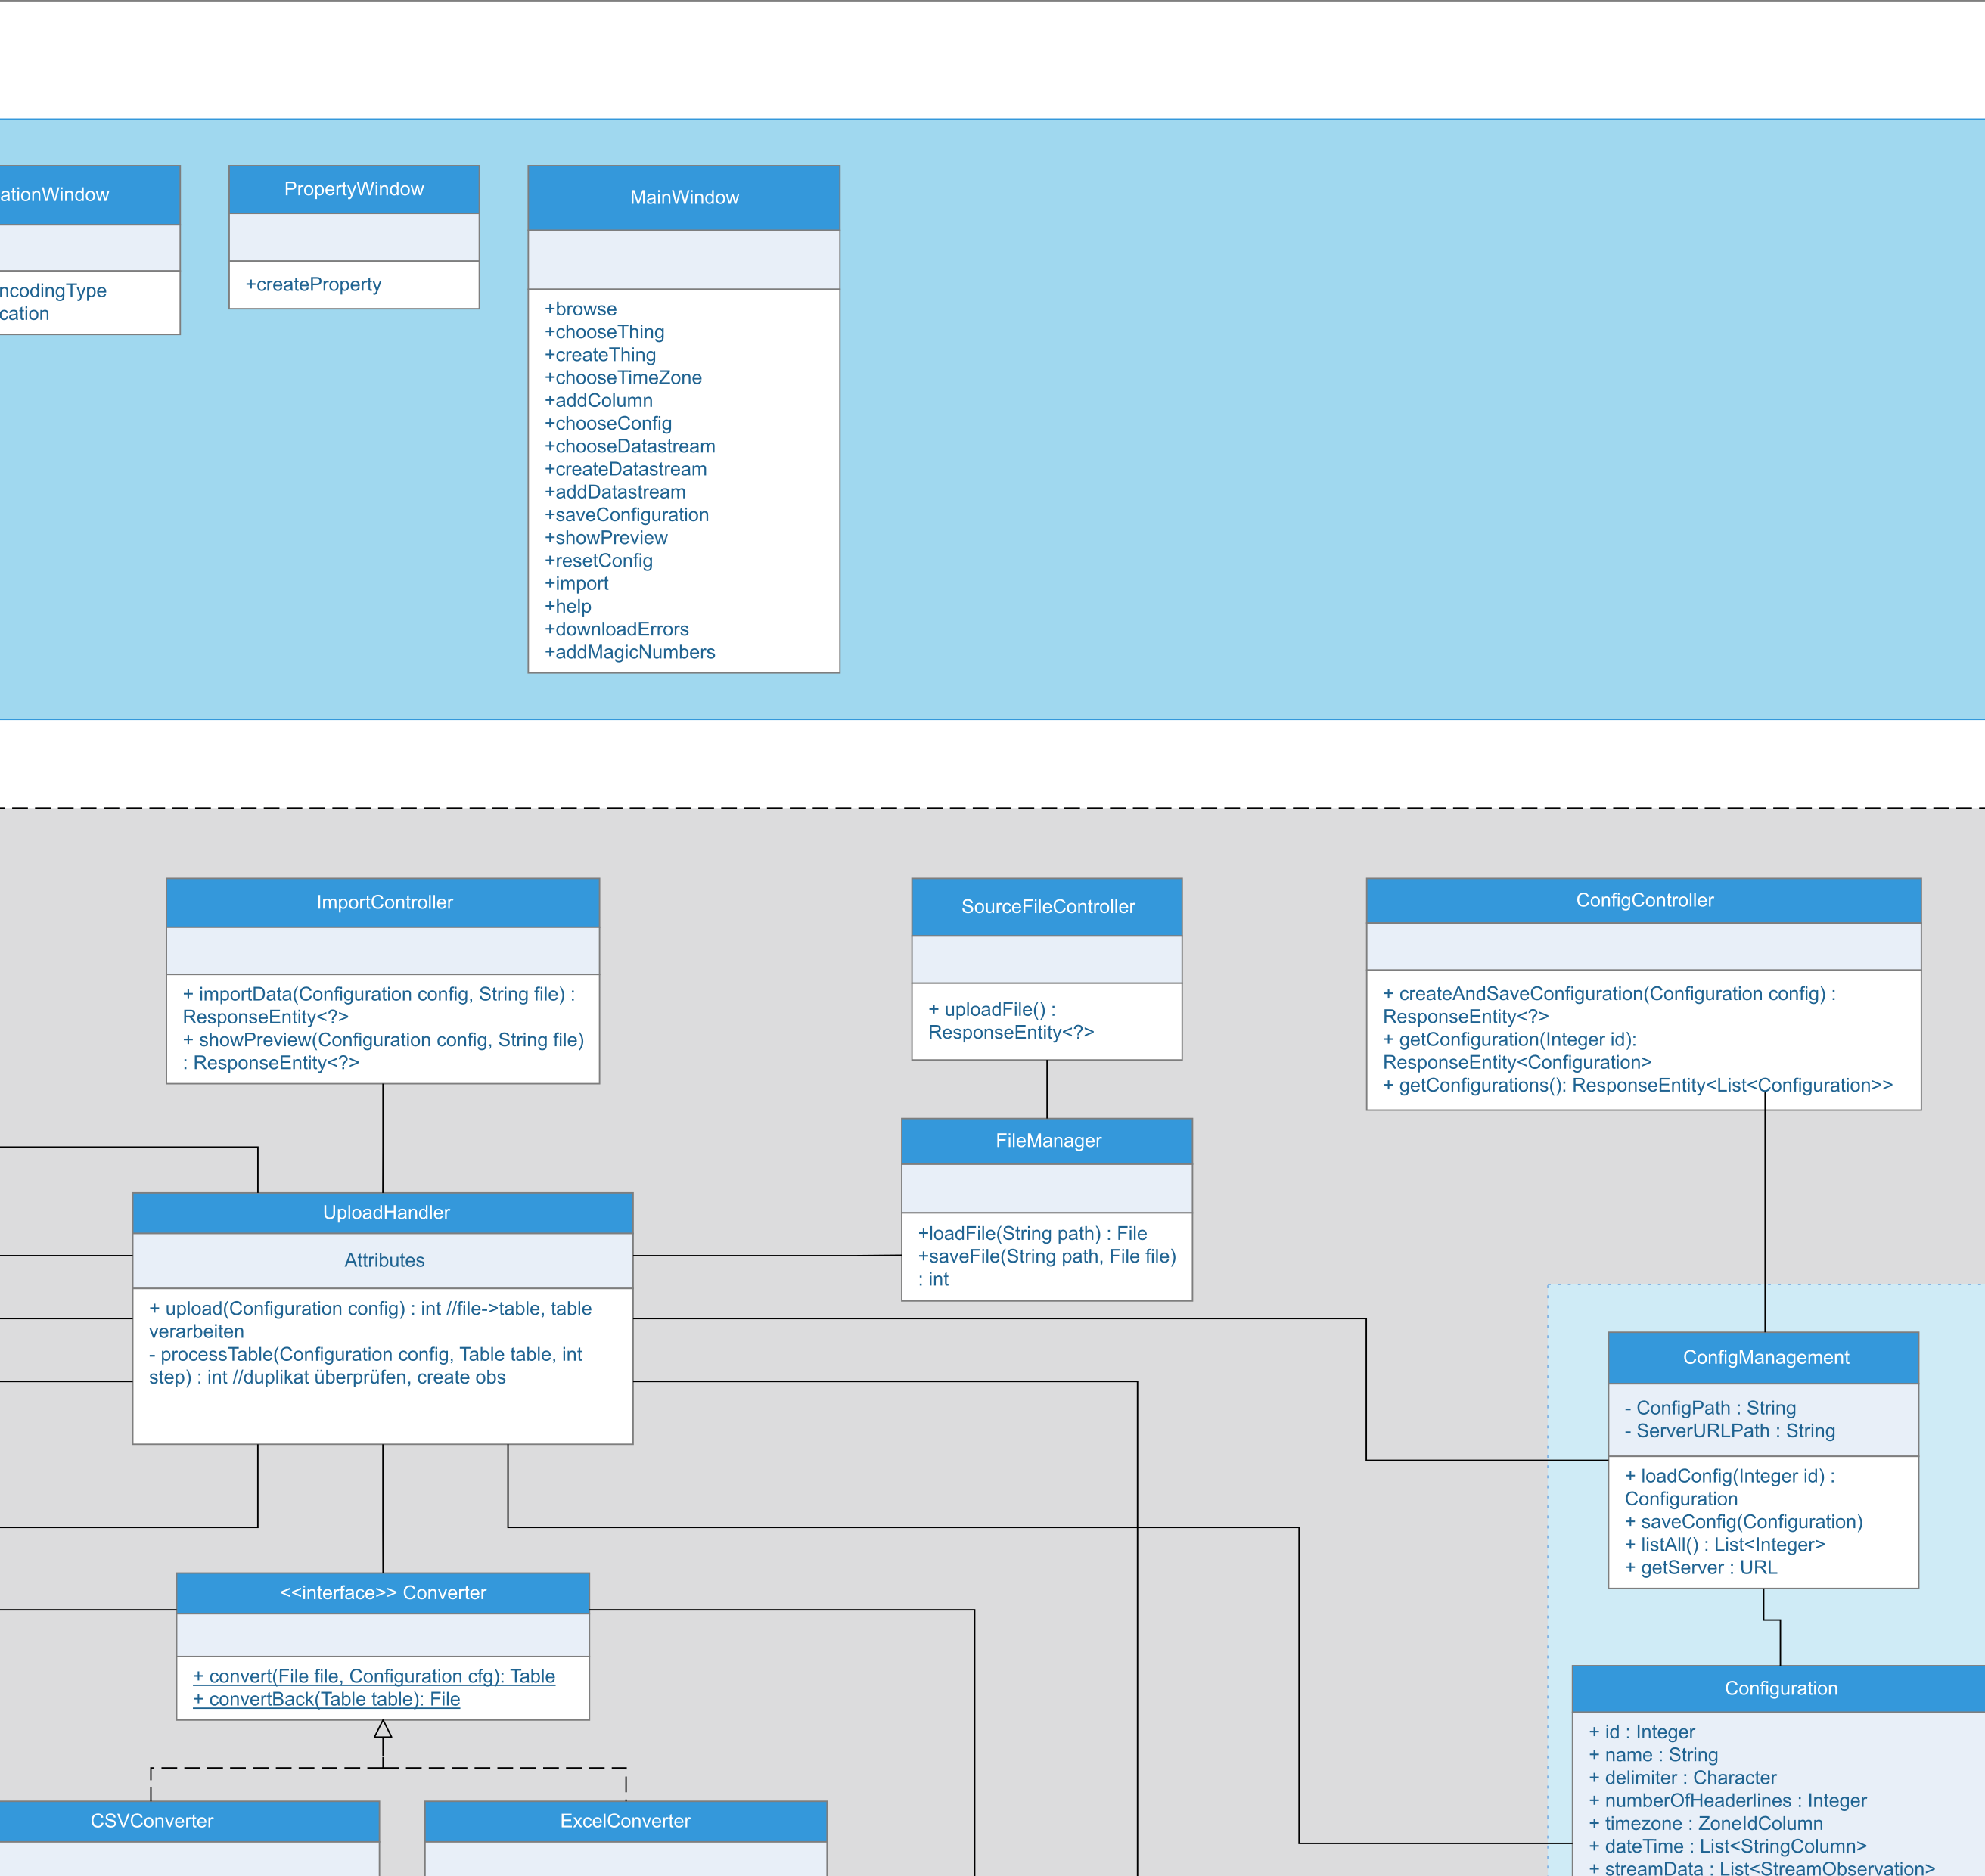
\includegraphics[scale=0.4]{uml/screenshots/frithjof/slice_0_2}
\caption{Ausschnitt 3 des Klassendiagramms}
\end{figure}
\clearpage

\begin{figure}[!h]
\centering
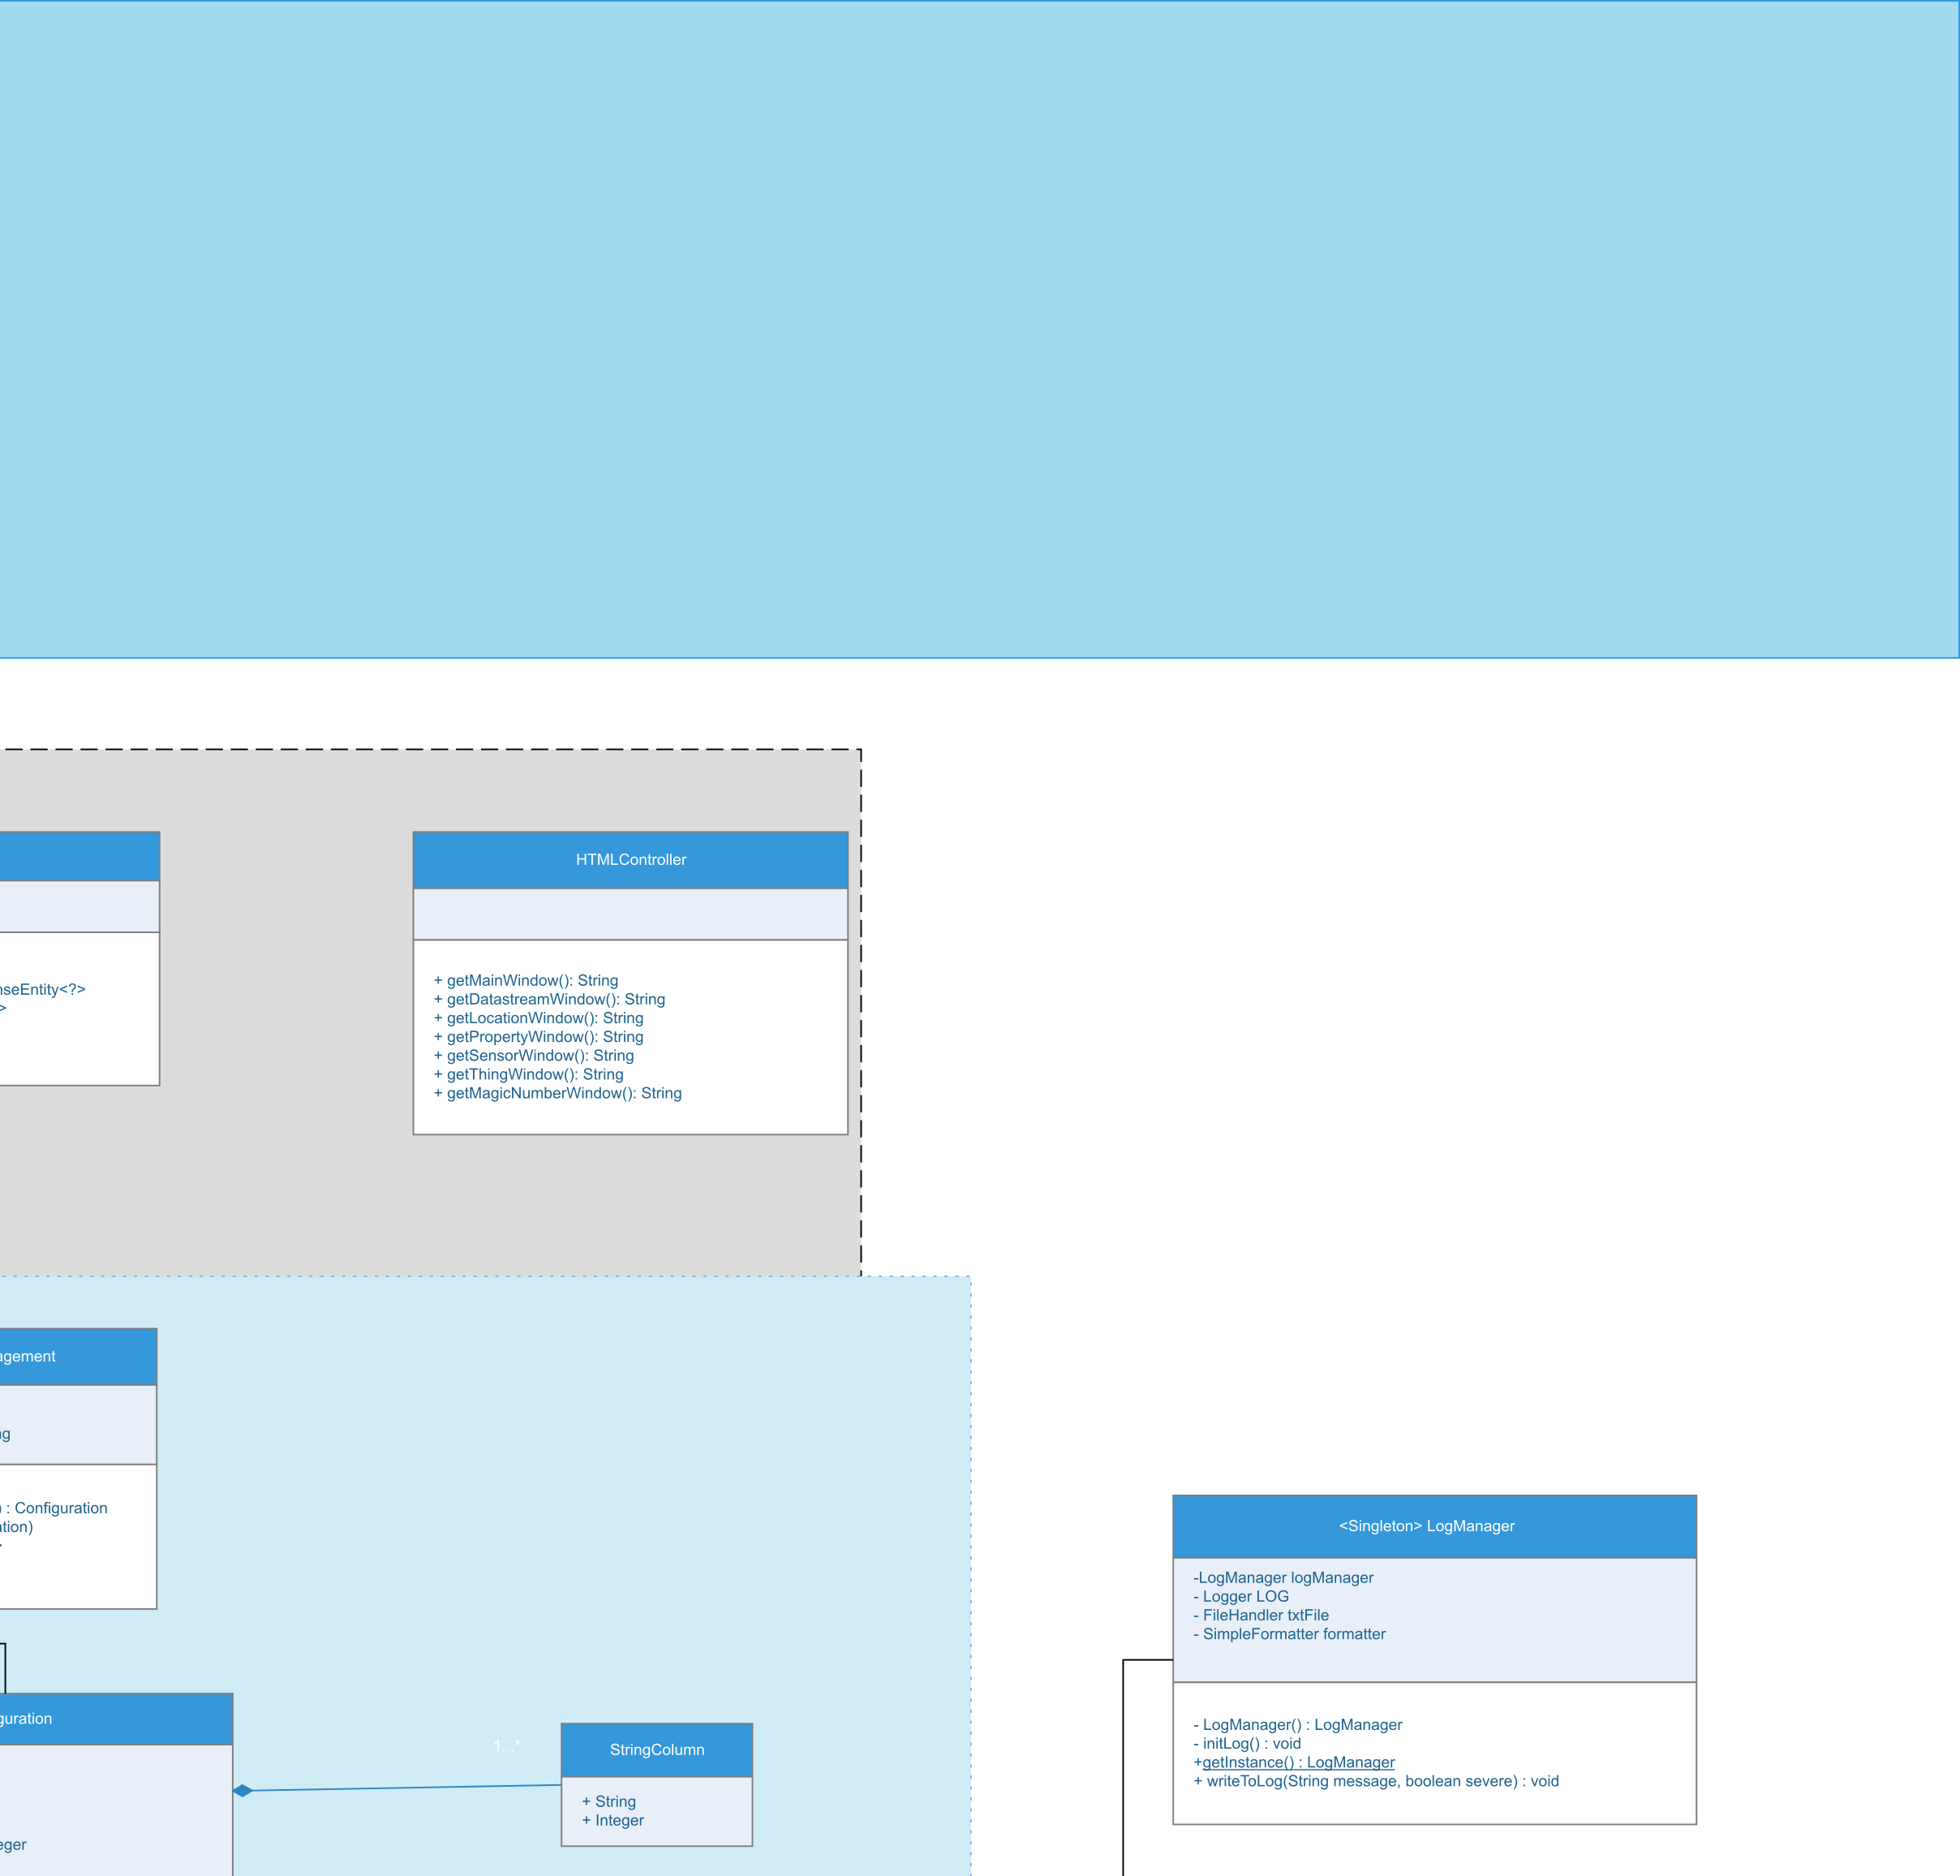
\includegraphics[scale=0.4]{uml/screenshots/frithjof/slice_0_3}
\caption{Ausschnitt 4 des Klassendiagramms}
\end{figure}
\clearpage

\begin{figure}[!h]
\centering
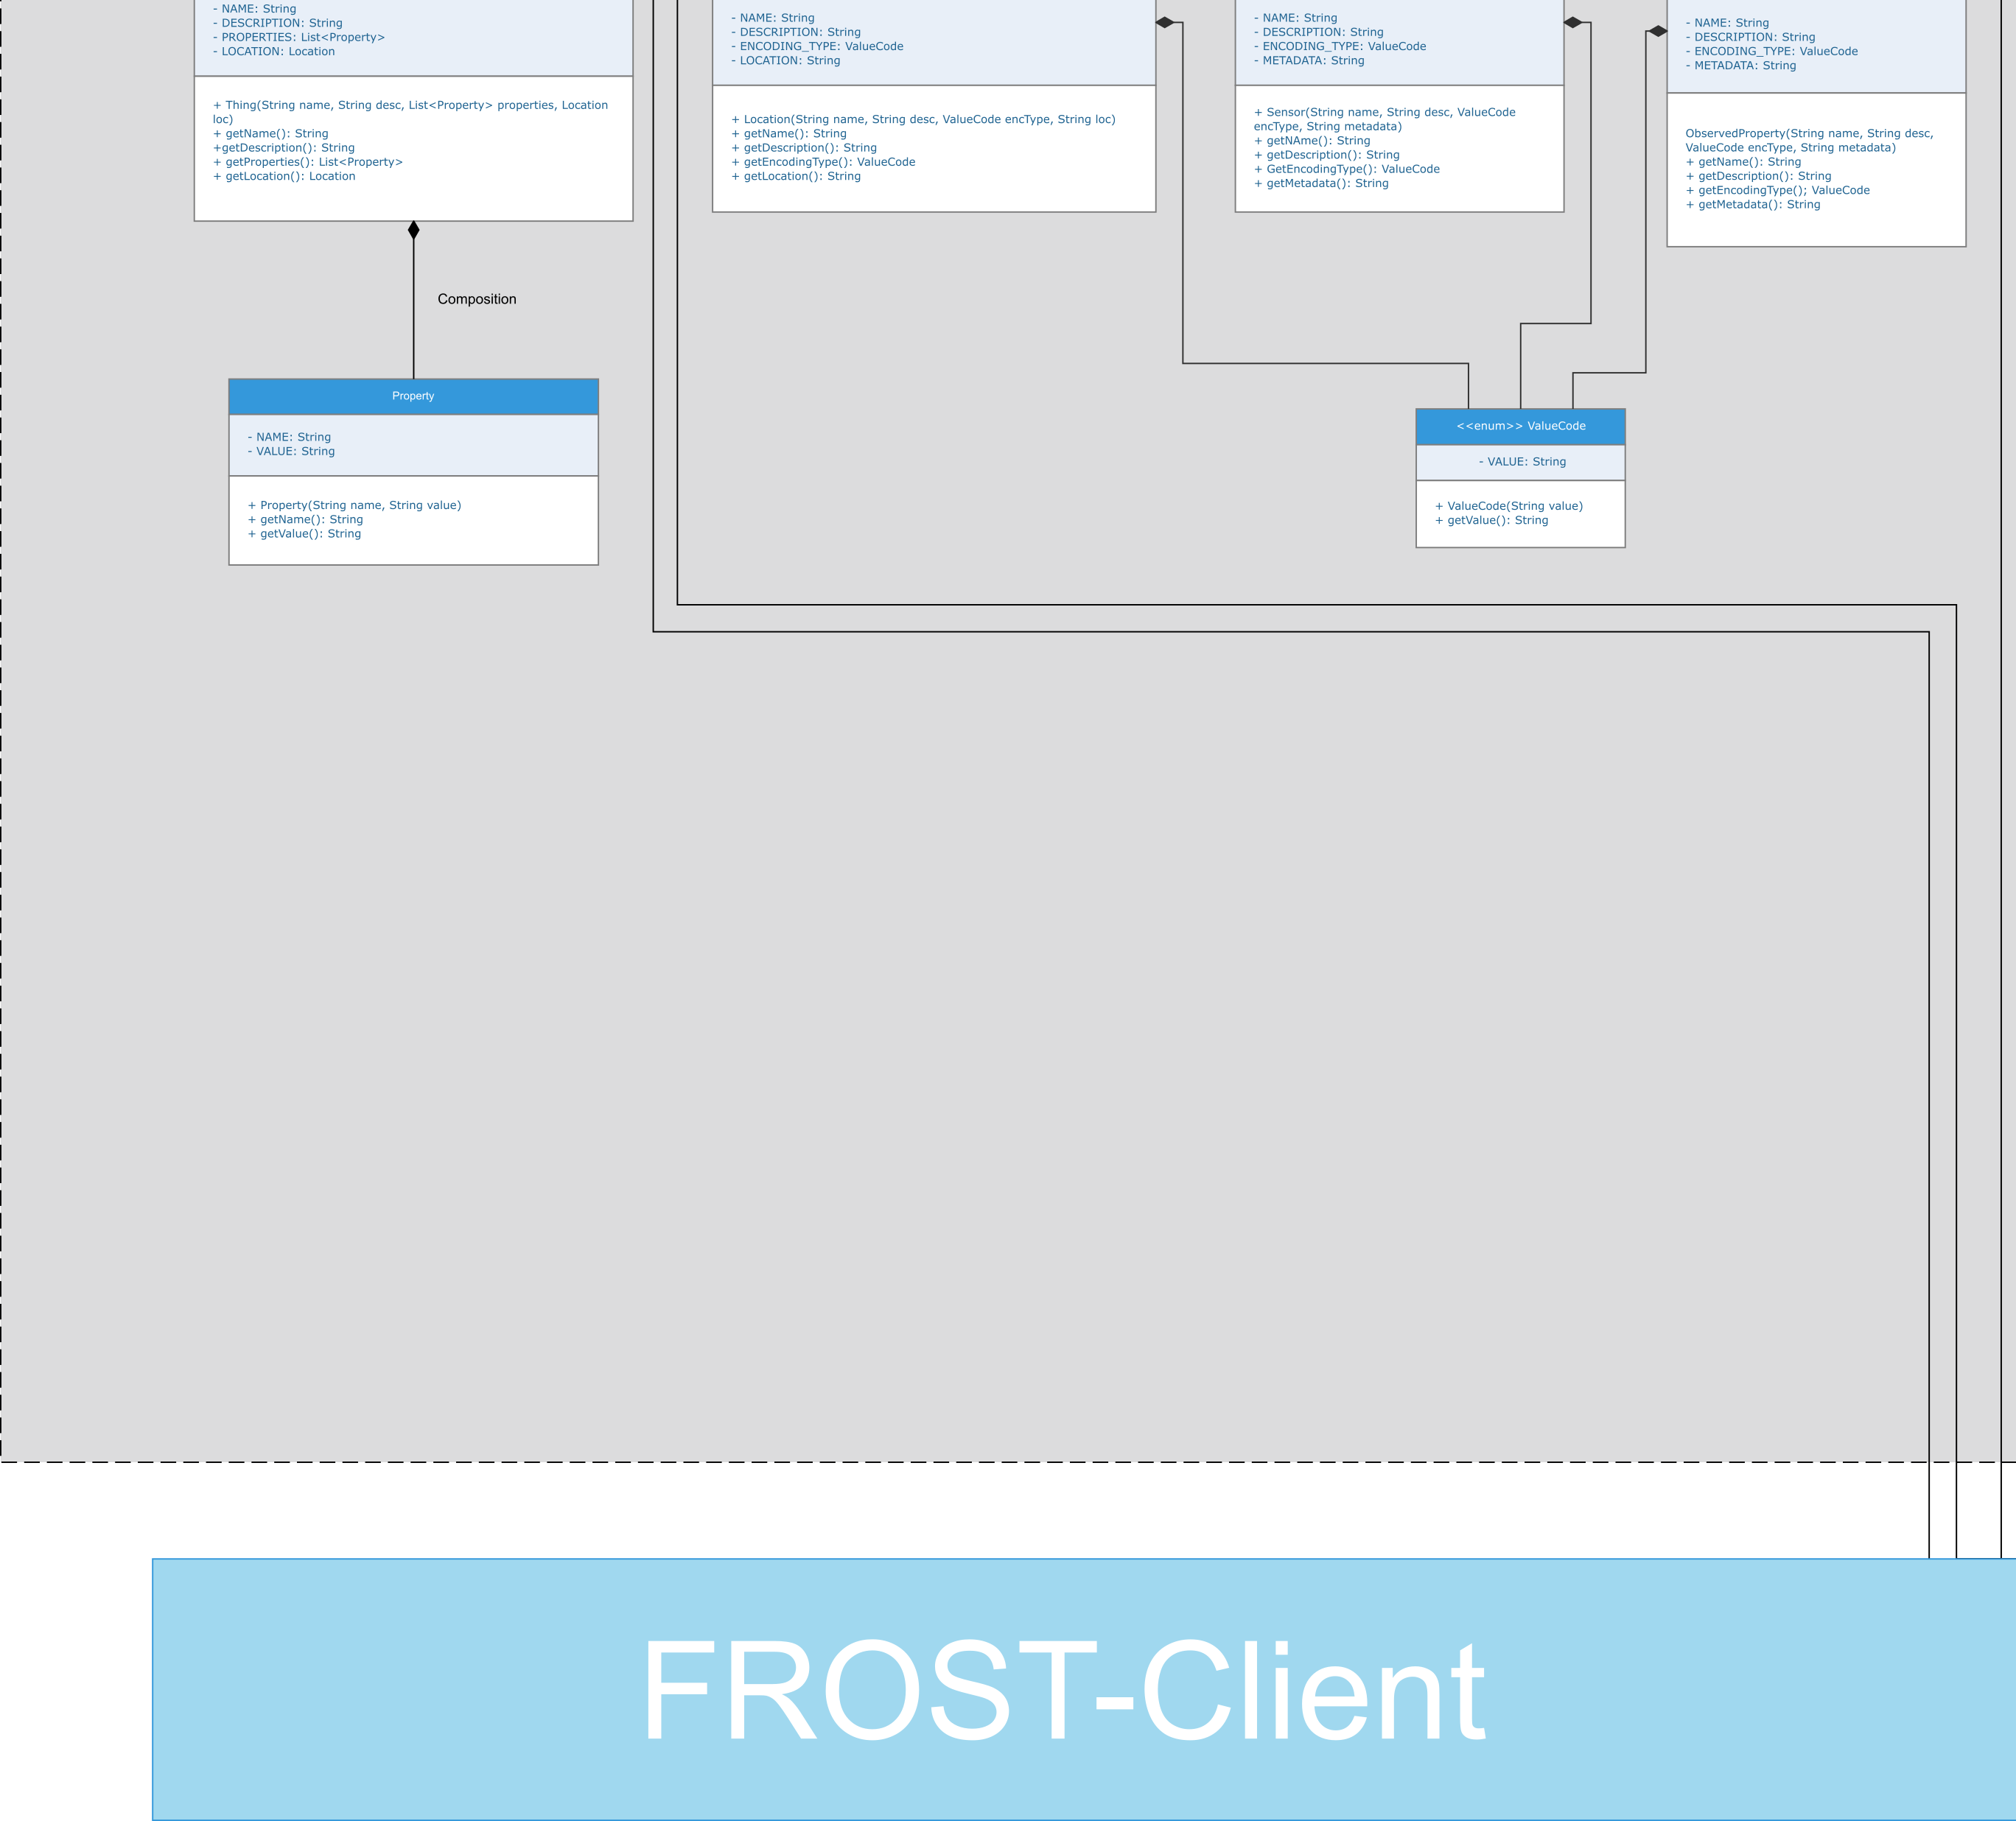
\includegraphics[scale=0.4]{uml/screenshots/frithjof/slice_1_0}
\caption{Ausschnitt 5 des Klassendiagramms}
\end{figure}
\clearpage

\begin{figure}[!h]
\centering
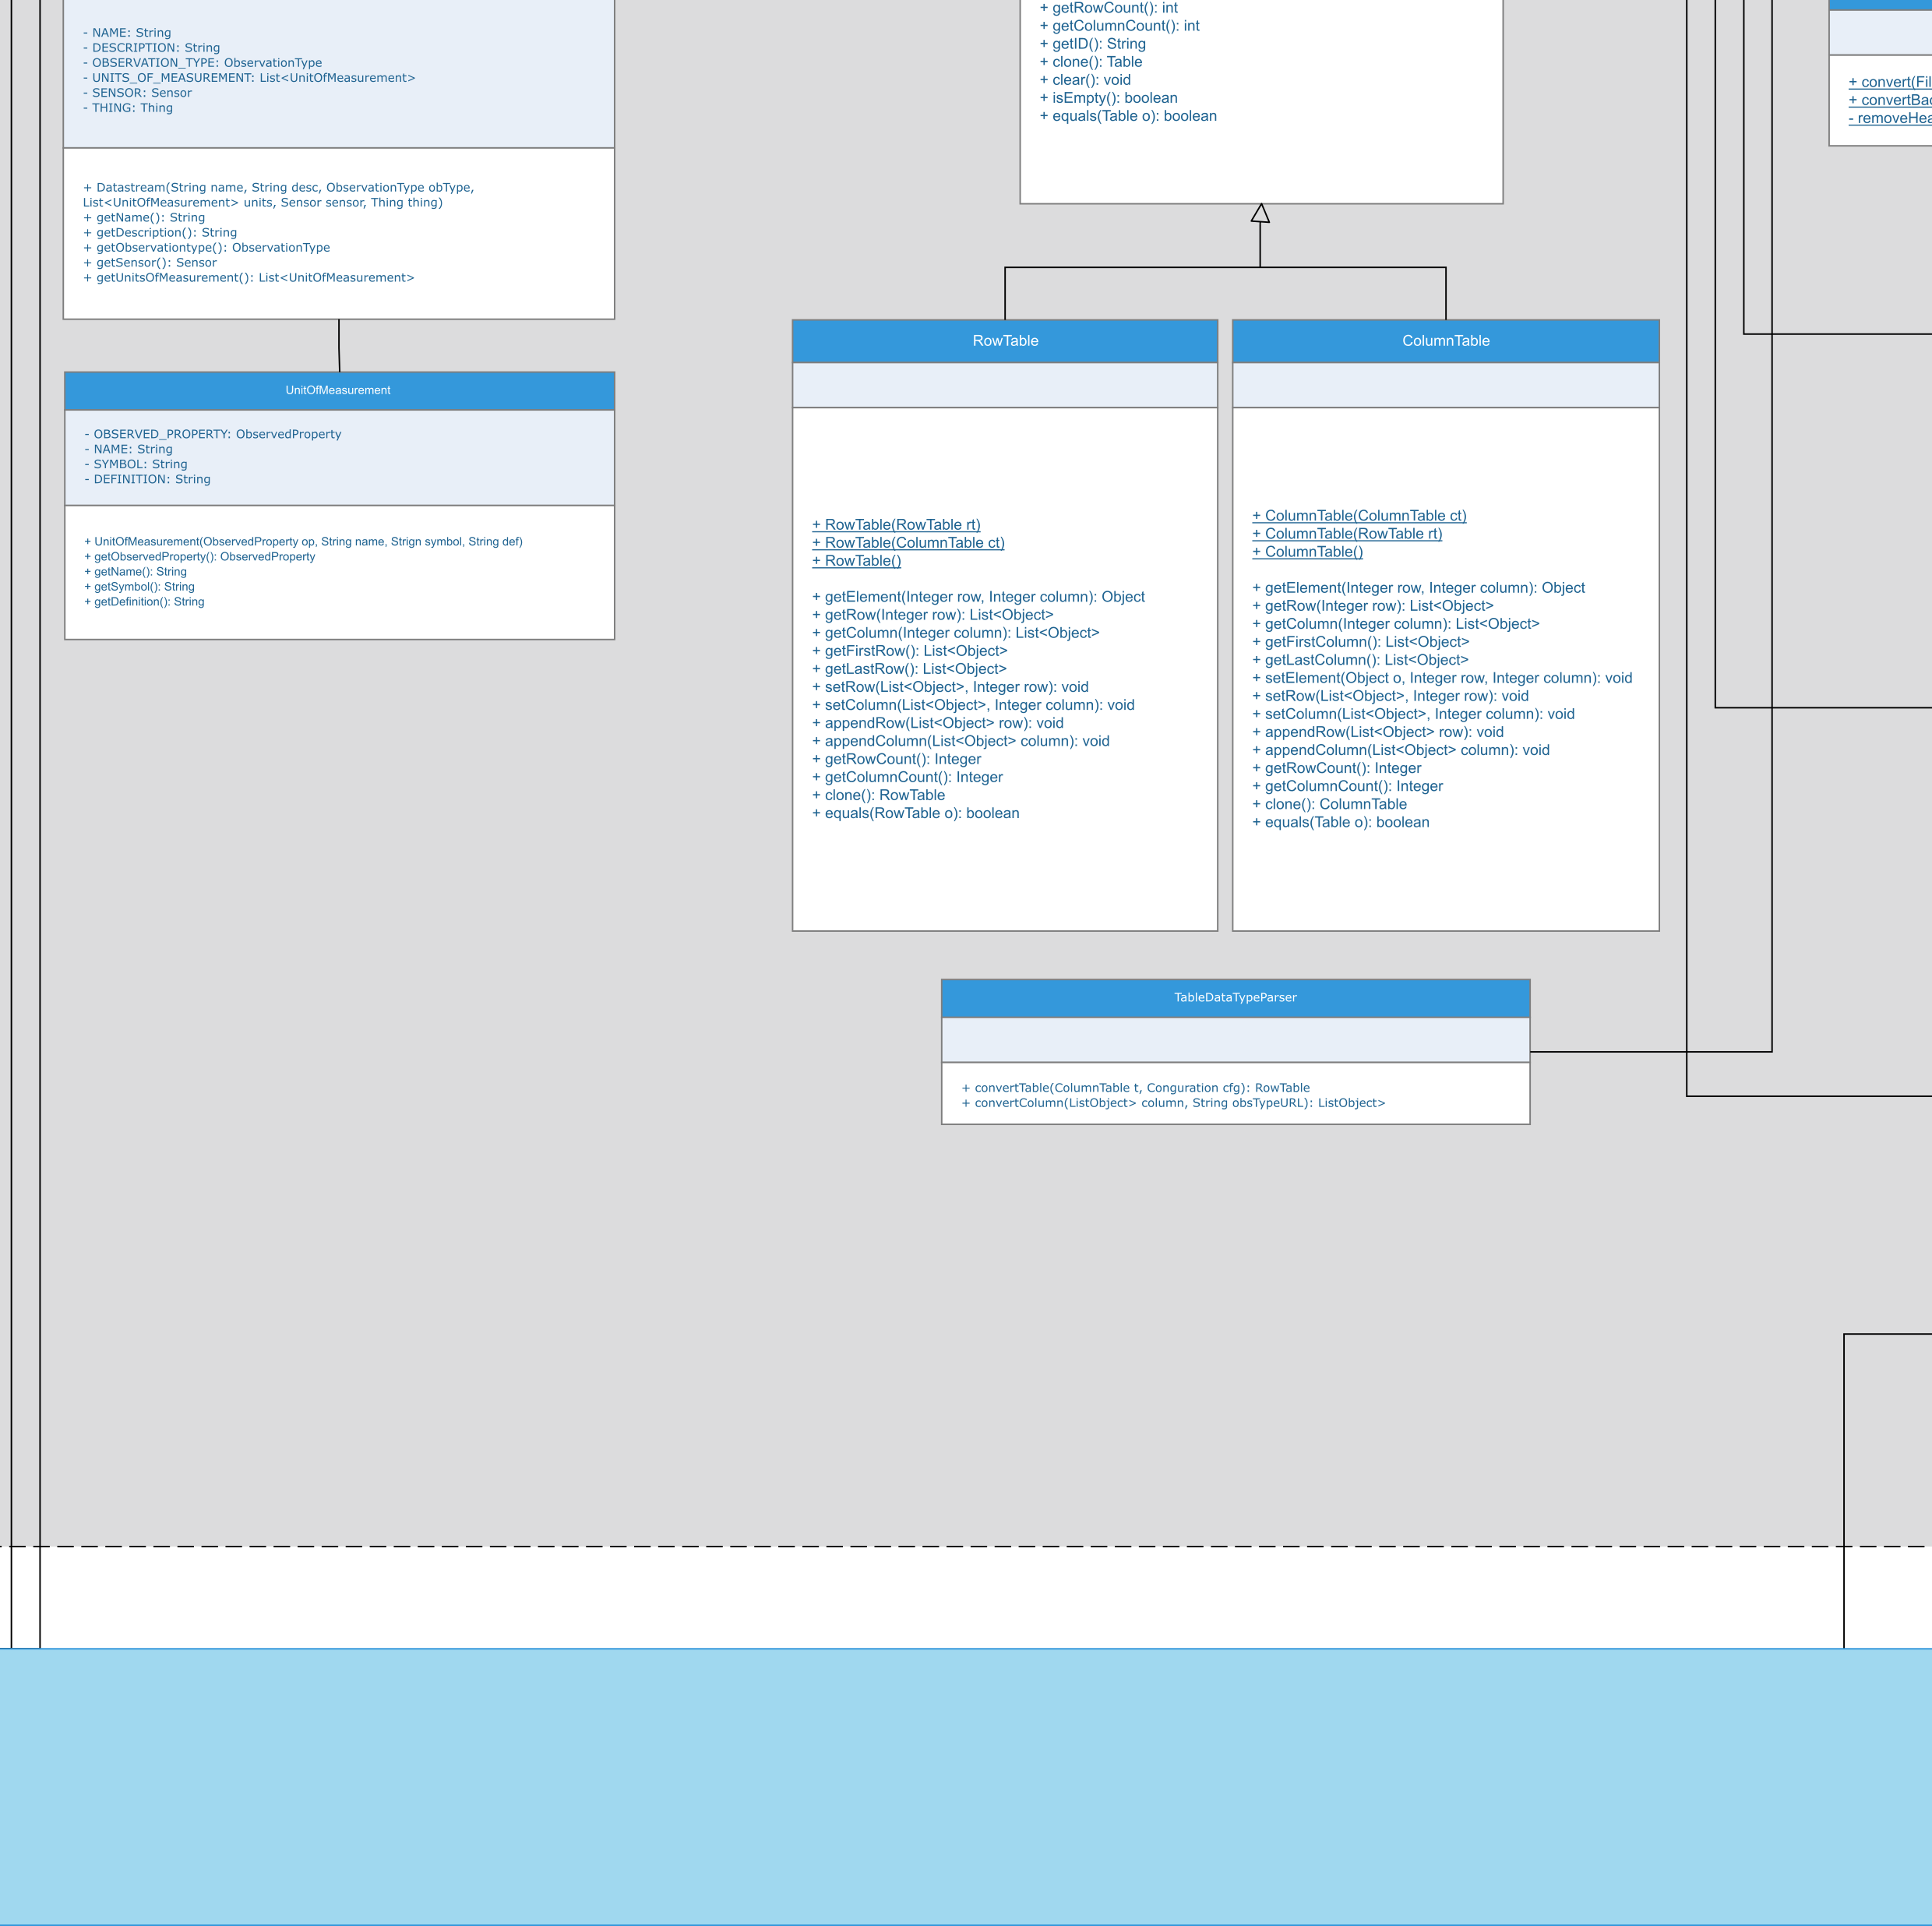
\includegraphics[scale=0.4]{uml/screenshots/frithjof/slice_1_1}
\caption{Ausschnitt 6 des Klassendiagramms}
\end{figure}
\clearpage

\begin{figure}[!h]
\centering
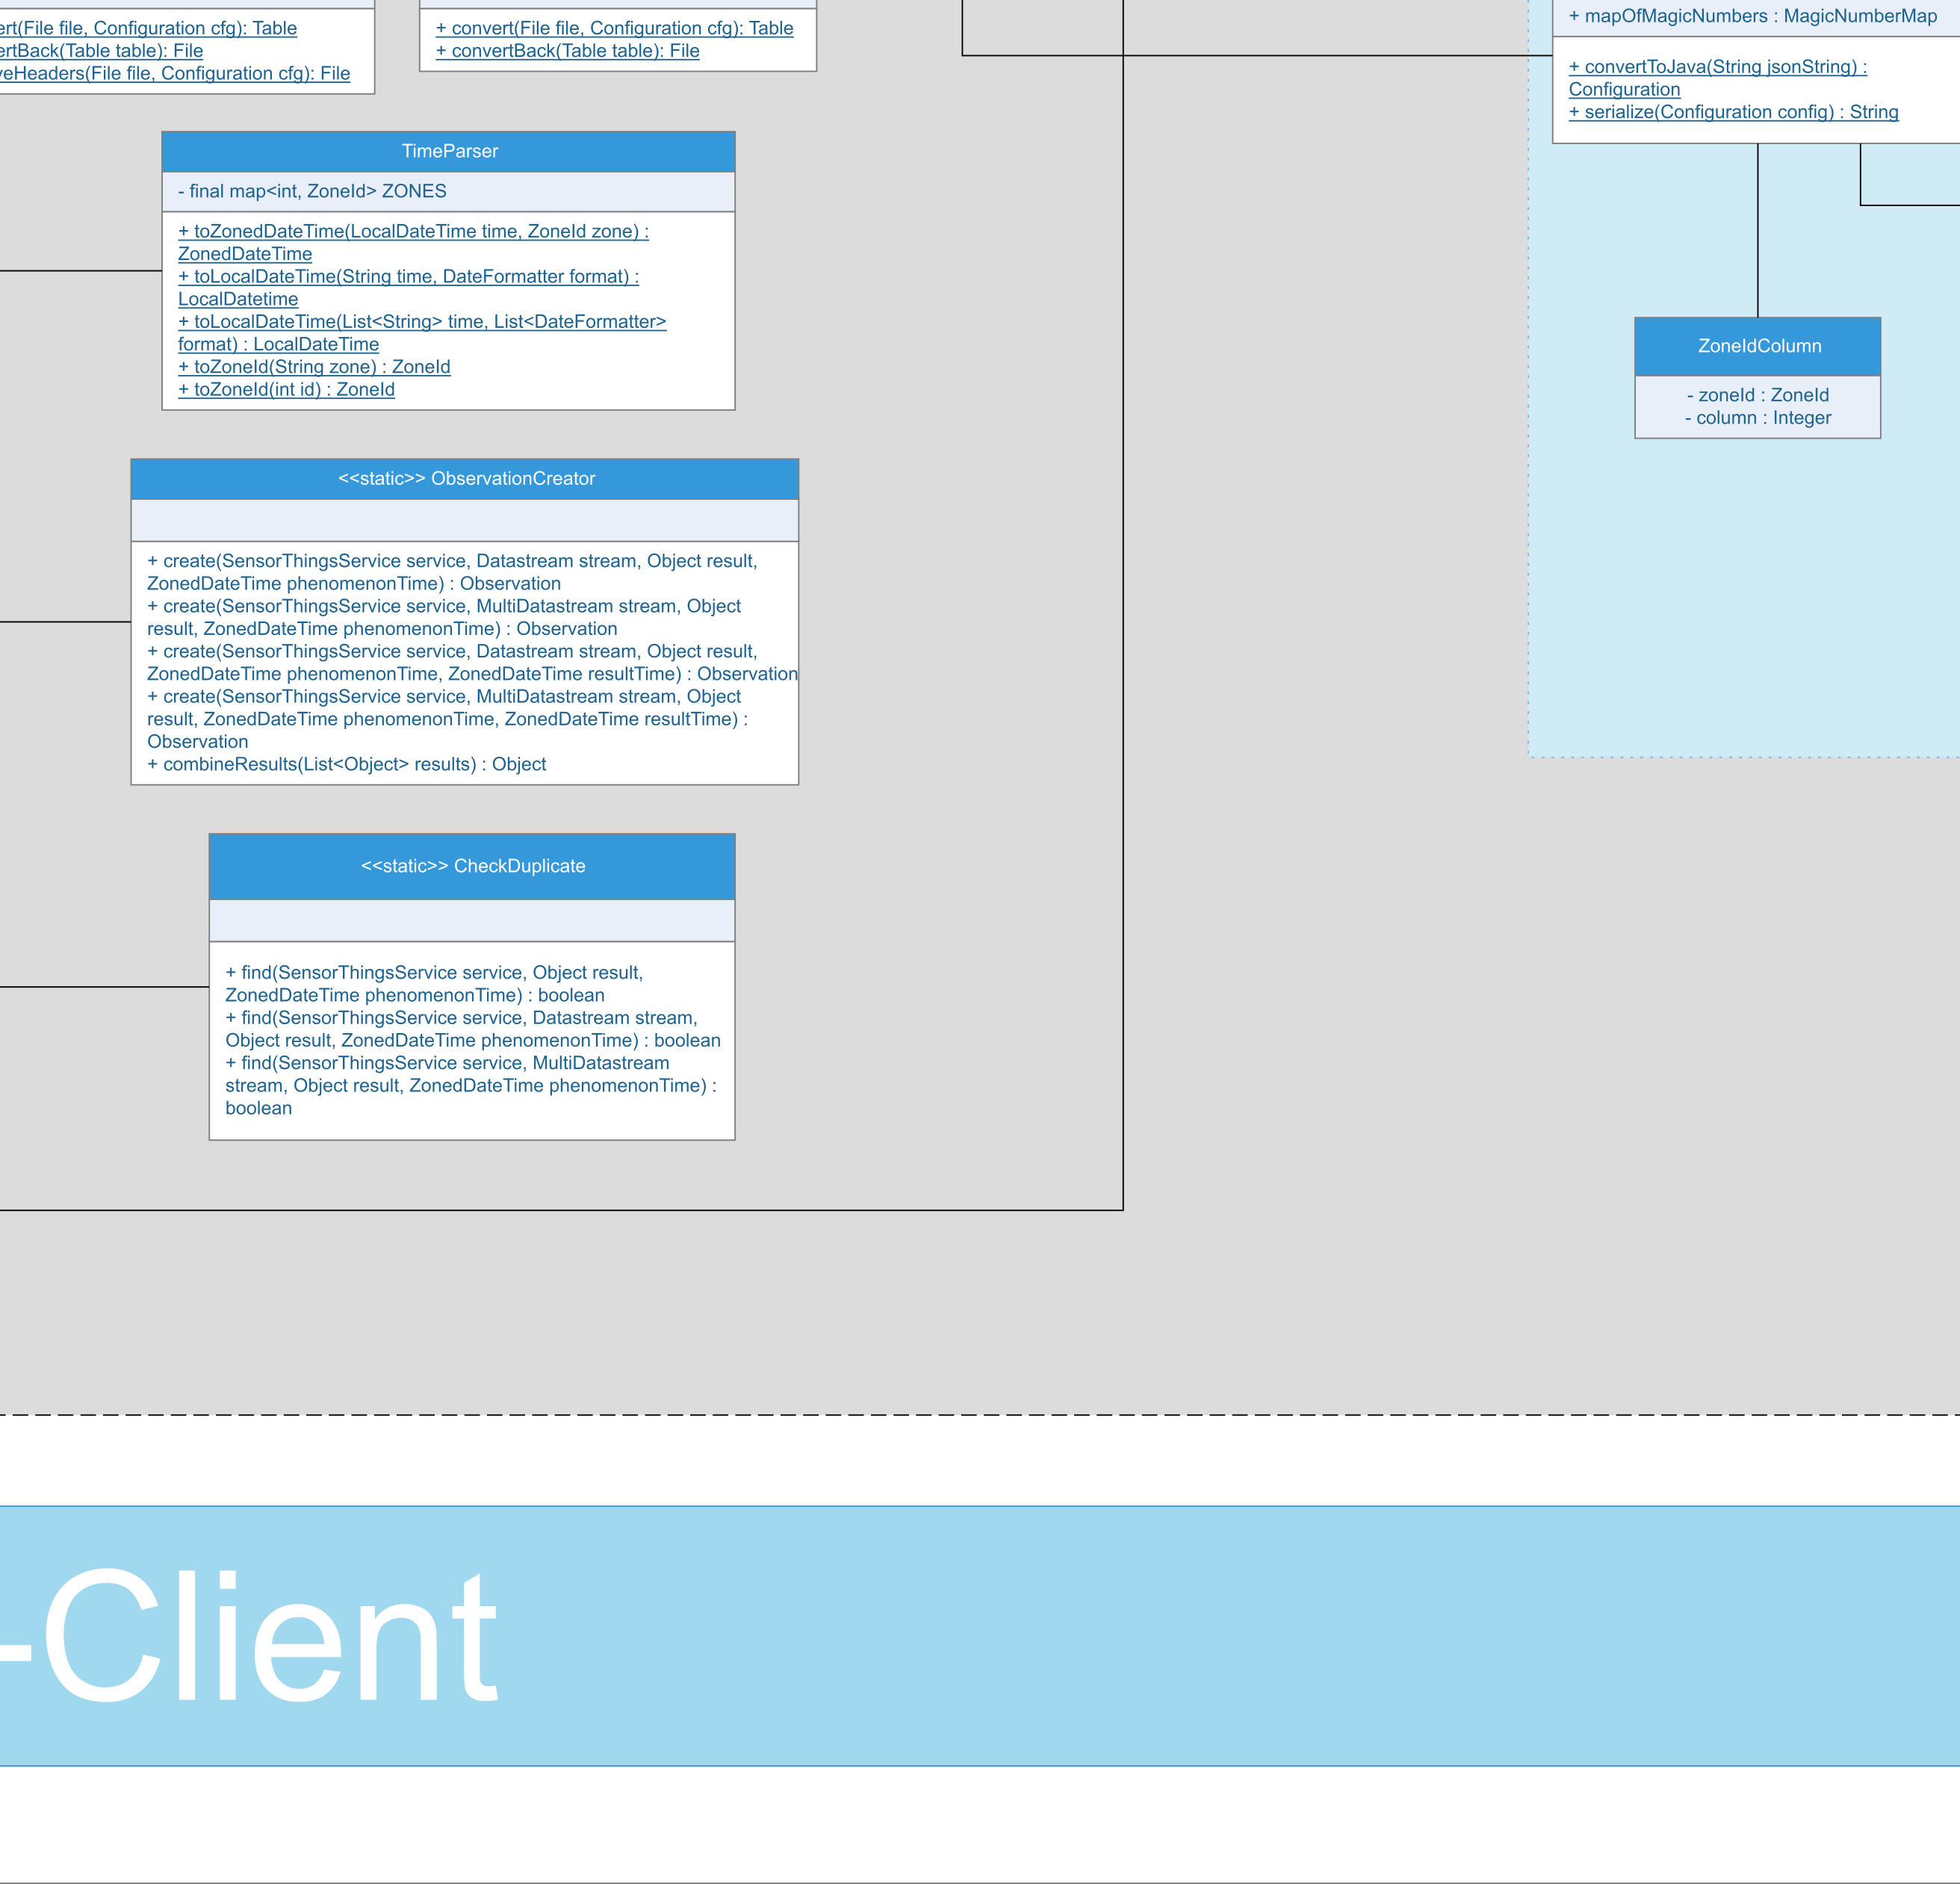
\includegraphics[scale=0.4]{uml/screenshots/frithjof/slice_1_2}
\caption{Ausschnitt 7 des Klassendiagramms}
\end{figure}
\clearpage

\begin{figure}[!h]
\centering
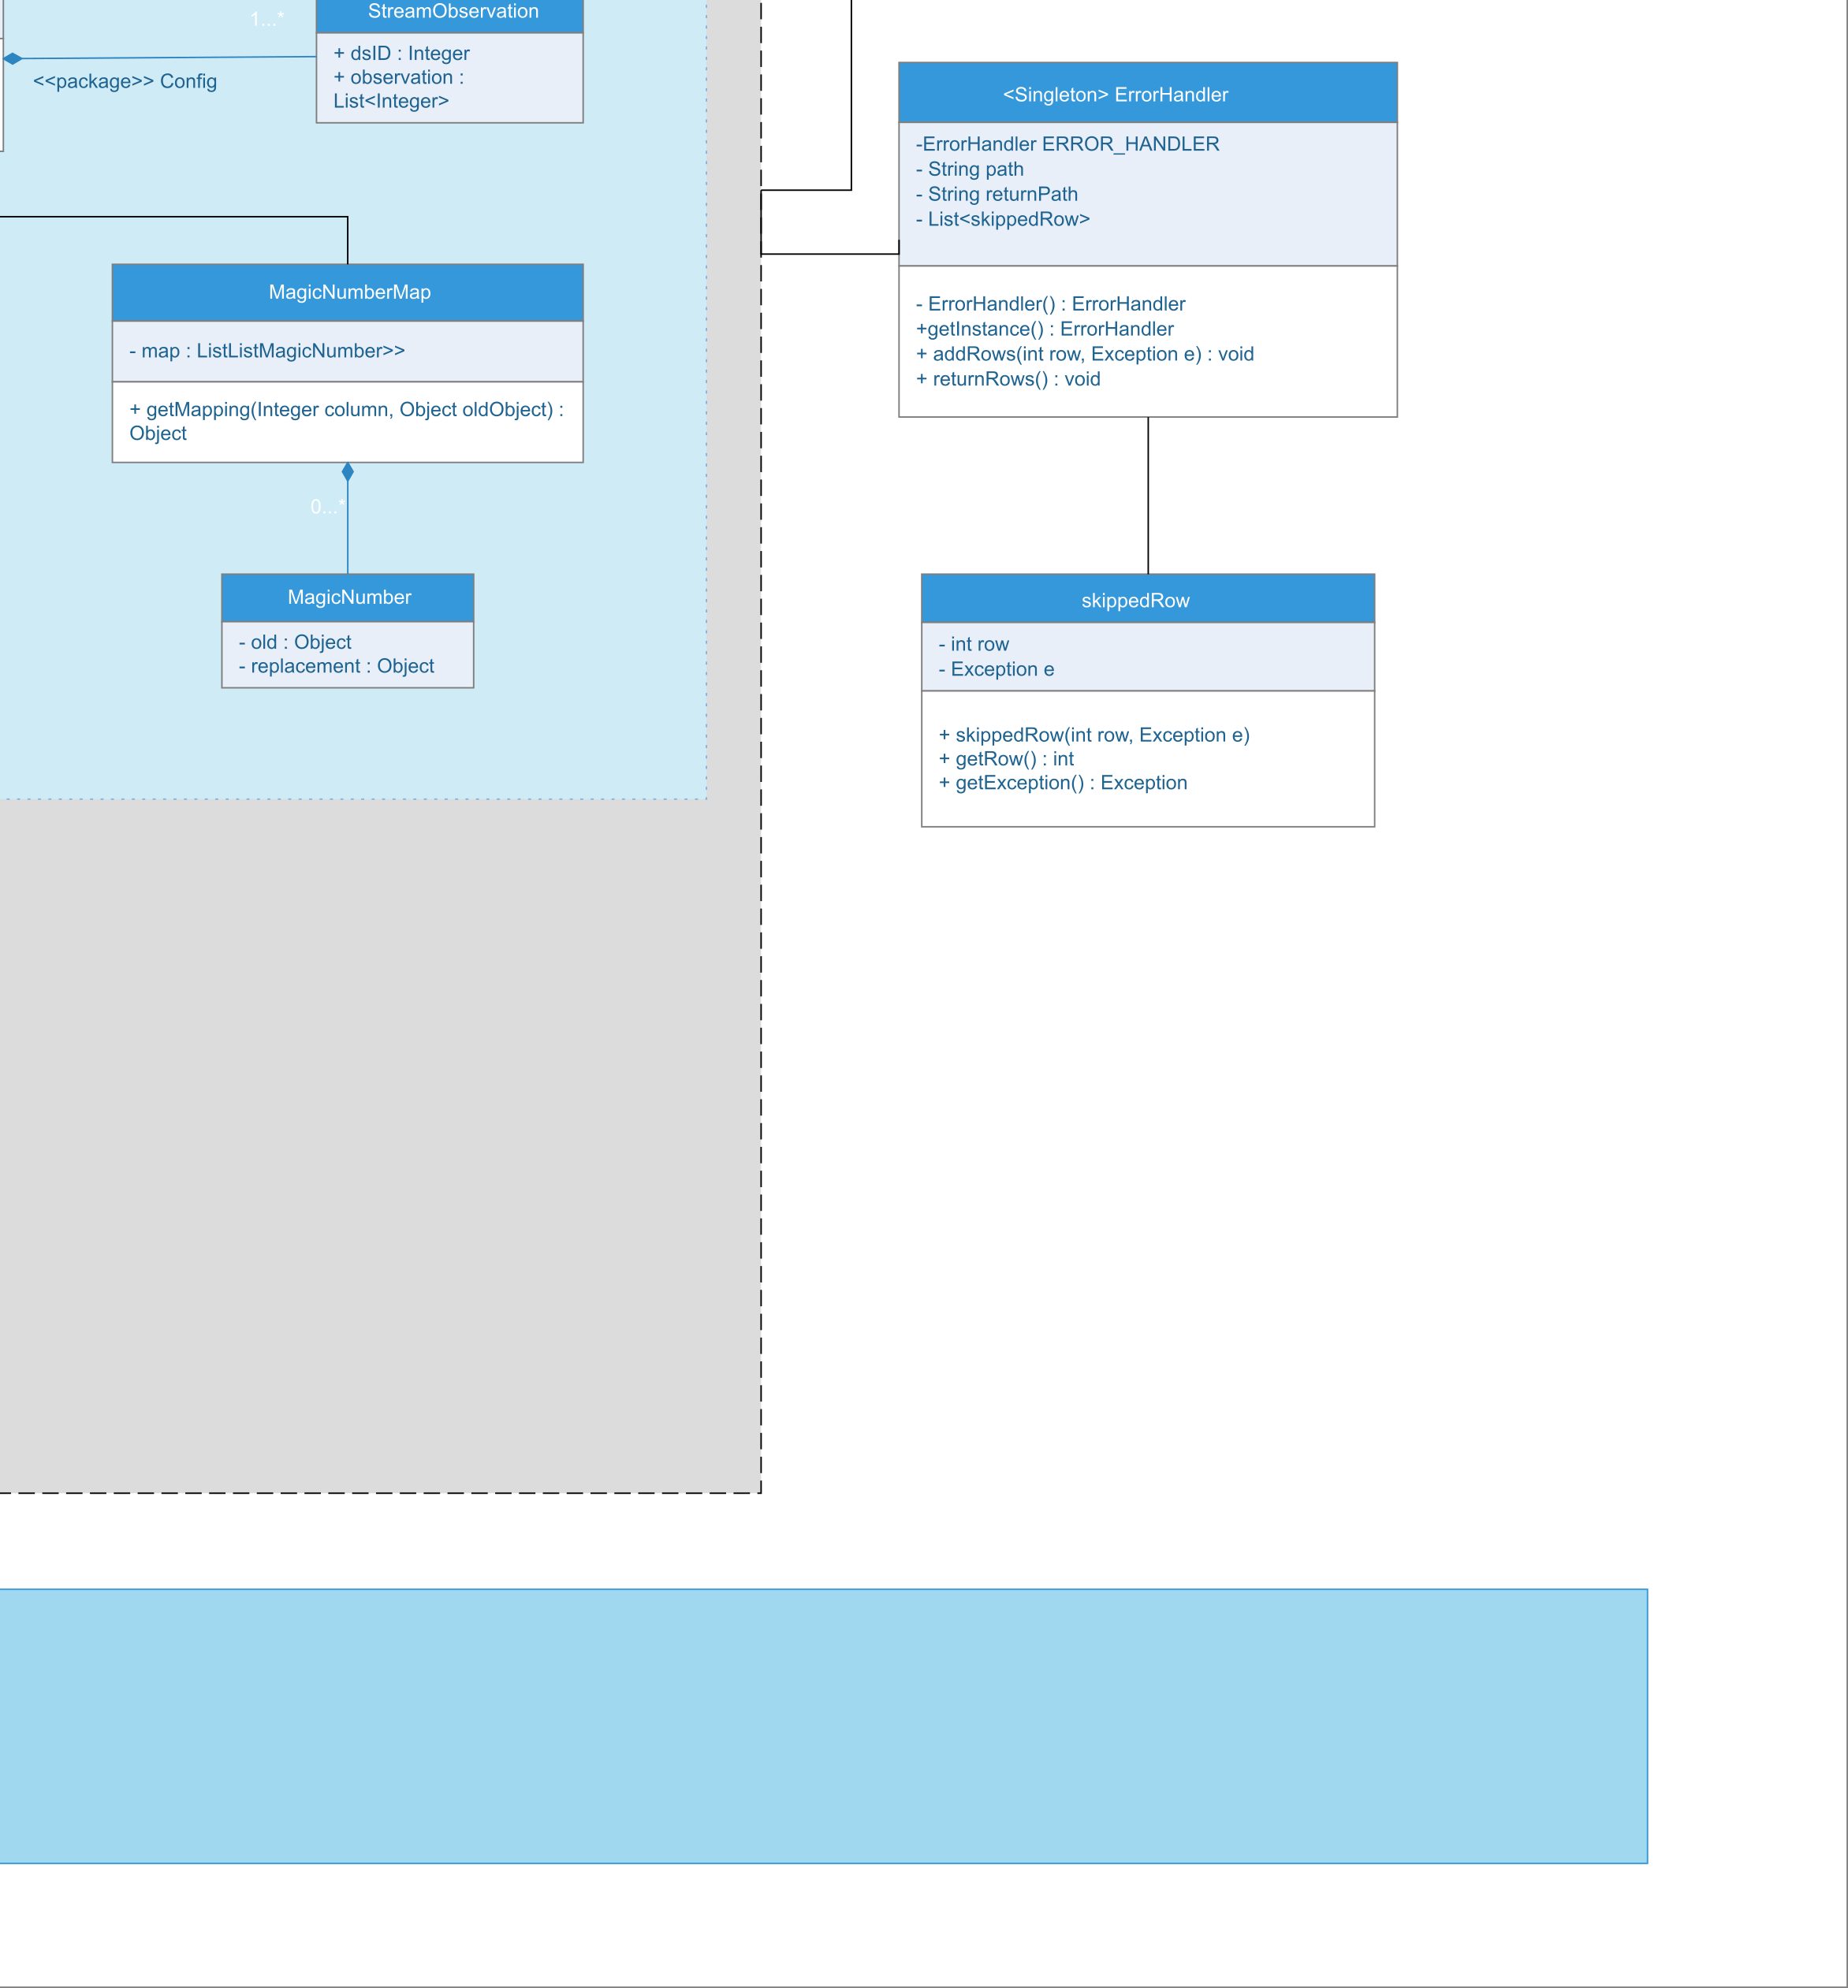
\includegraphics[scale=0.4]{uml/screenshots/frithjof/slice_1_3}
\caption{Ausschnitt 8 des Klassendiagramms}
\end{figure}